\documentclass{article}

\usepackage{url}
\usepackage{color}
    \definecolor{darkblue}{RGB}{6,69,173}
\usepackage{hyperref}
    \hypersetup{
        colorlinks=true,
        linkcolor=darkblue,
        urlcolor=darkblue
    }
\usepackage{graphicx}
\usepackage{listings}

\begin{document}

\title{%
    Git Gud \\
    \large Or How To Never Lose Your Work Again}
\author{Cat Flynn}

\maketitle
\pagenumbering{gobble}
\newpage
\tableofcontents
\newpage
\pagenumbering{arabic}

\section{Introduction}
I'm sure all of us have lost a project or two thanks to unexpected failures, like a UE update corrupting your project beyond recognition or your expensive motherboard suddenly crapping out after only a year and a half. We didn't back it up because we're \textit{lazy}, and \textit{maybe I'll do it later}. It's easy to make excuses, and to say what you should have done in hindsight, but the truth is that \textit{there is a better way}.

\section{What's Git?}
Git is a tool used by developers primarily as insurance, and secondarily as a system for collaboration. It tracks incremental updates to a project and distributes them between multiple locations, such as servers and other developers' machines. Imagine setting checkpoints in your project every time you fix a bug, or implement a feature. You can track what work you did and when you did it, with the bonus of having your precious work safely out of harm's way if your PC explodes!

\section{Alright, I'm sold. How do I use Git?}
Start by downloading Git from \href{https://git-scm.com/}{git-scm.com}, and installing it. The default options should be totally fine, so go ahead and click right through. Once you're done instaling, you'll be greeted by a \textit{hacker} looking terminal (\ref{fig:terminal}). Don't be scared of it, there are only a few commands you'll need to know to be able to use Git effectively. The command line is fun, trust me!

\begin{figure}
    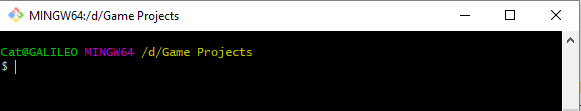
\includegraphics[width=\linewidth]{images/terminal.png}
    \caption{\textit{*hacker voice*} I'm in}
    \label{fig:terminal}
\end{figure}

\paragraph{}
The main thing to note the yellow text, which is the location in your filesystem that Git is currently running in. You can use the command \texttt{ls} to list the files and folders in this directory, and \texttt{cd} to navigate in and out of these folders. The command \texttt{cd ..} will take you to the current folder's parent; for example, running \texttt{cd ..} in the prompt shown in \ref{fig:terminal} would take me to the \texttt{/d/} folder. Lastly, the \texttt{clear} command will clear the screen, giving you a blank terminal to work with.

\paragraph{}
Before we get into using Git, let us take a moment to properly configure it. We need to give it an email and a name, so that it can attach this information to any work we do. This is required, and Git won't work without it. Run the \texttt{git config} commands as shown in \ref{fig:config} to accomplish this.

\begin{figure}
    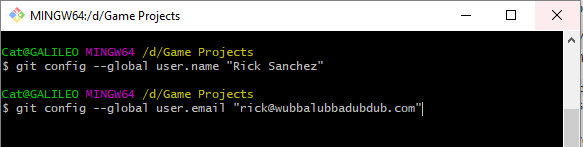
\includegraphics[width=\linewidth]{images/config.png}
    \caption{Git configuration.}
    \label{fig:config}
\end{figure}

\paragraph{}
Great! Now it's time to set up a project. This guide is primarily aimed at users of the Unity game engine on Windows, but the steps outlined will work for any project, on any system. Go ahead and create your project as normal (or you can use an existing project) and get it open in File Explorer.

\paragraph{}
Before we continue, make sure you've enabled file extenations and hidden folders in File Explorer. These options are accessed from the View tab. Right click anywhere in this folder and select `Git Bash here'. A terminal like the one we opened earlier should appear, and you'll notice the yellow path matches the filepath of your project.

\begin{figure}
    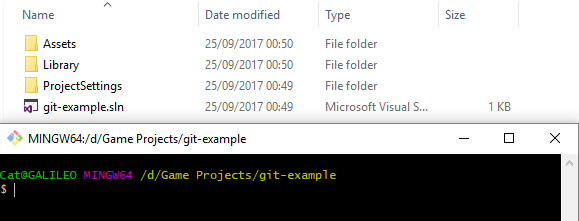
\includegraphics[width=\linewidth]{images/pre-init.png}
    \caption{Opening Git Bash in a particular folder.}
    \label{fig:pre-init}
\end{figure}

\paragraph{}
Now run the command \texttt{git init}. This command creates a `repository' in this folder. Git stores the repository state in this folder. The repository is how Git is able to share your project with others. It builds a history of changes, tracking who changed what in which files and when they did it. 

\begin{figure}
    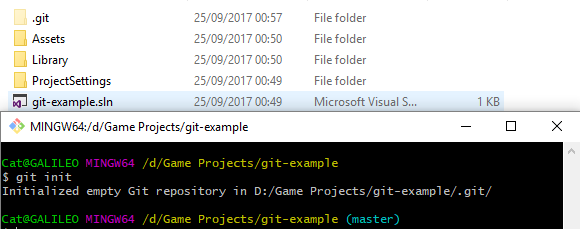
\includegraphics[width=\linewidth]{images/post-init.png}
    \caption{A project with an initialised Git repository.}
    \label{fig:post-init}
\end{figure}

\paragraph{}
You'll immediately notice a couple of things. First, there's now a faded-looking \texttt{.git} folder (\ref{fig:post-init}) sitting alongside your project. This is where Git stores whatever it needs to worry about, you shouldn't ever have to go looking in there. However, you should note that this folder needs to stay in the project root for Git to work properly. Second, there is now a blue \texttt{(master)} label after the filepath in Git's command prompt. This is the name of the current \textit{branch} you're on. Since Git stores projects as a tree, it must have at least one branch. The \texttt{master} branch is created be default in a Git repository. You can rename, add and remove branches from a repository at your leisure, but that isn't in the scope of this guide. One branch is plenty for now! As a handy tip, if there is no branch in the command prompt then that means there's no repository present either.

\begin{figure}
    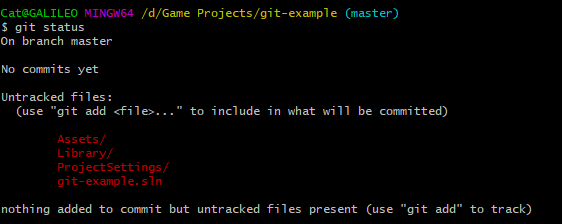
\includegraphics[width=\linewidth]{images/status.png}
    \caption{Output of \texttt{git status}.}
    \label{fig:status}
\end{figure}

\paragraph{}
Now, let's make our first commit! Start out by running the command \texttt{git status} to view the current state of the repository. As seen in figure \ref{fig:status} this command outputs the folders in our project, highlighted in red because they're currently not being tracked by Git. So let's do that! Run \texttt{git add *} to tell Git to start tracking everything. You can also specify particular paths to add only specific files or folders, such as \texttt{git add Assets/}.

\begin{figure}
    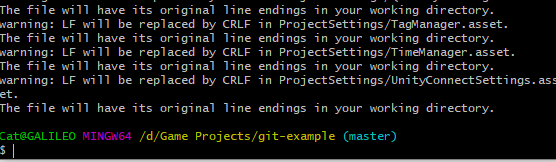
\includegraphics[width=\linewidth]{images/add-out.png}
    \caption{Output of \texttt{git add}.}
    \label{fig:addout}
\end{figure}

\paragraph{}
Depending on the platform you're using, \texttt{git add} will spit out a bunch of output(figure \ref{fig:addout}), but this isn't anything to worry about. Run \texttt{git status} again to see how we've updated the state of the repository.Figure \ref{fig:statusgreen} shows a bunch of filenames in green. These files are now being tracked by Git. Since we added everything in our root directory, every file in our project is being tracked. Later, we'll talk about how to ignore particular files, such as those generated by the tools you're using, or build artifacts.

\begin{figure}
    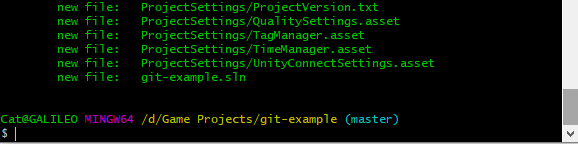
\includegraphics[width=\linewidth]{images/statusgreen.png}
    \caption{Files being tracked by Git after running \texttt{git add}.}
    \label{fig:statusgreen}
\end{figure}

\paragraph{}
Now that Git is tracking our files, it's time to actually save them! We'll do this by making a \texttt{commit}. A commit is a set of changes to a set of files. In this case, it's picking up the creation of all the project files, since it was just an empty repository before. Run the command \texttt{git commit \-m "initial commit"} to create a commit. The \texttt{\-m} flag allows you to specify a descriptive message explaining the changes you made such that you can understand the project history at a glance later, or try to track down bugs. \texttt{git commit} will produce more output, and you'll find that \texttt{git status} no longer shows anything in your \textit{working directory}, since the files haven't changed since committing. Run \texttt{git log} and you can see the commit you made, along with the name and email we configured earlier.

\paragraph{}
One last step before you can use Git to back up your projects! While you now have your project in a local repository, that won't do you any good if your computer dies. You can self-host Git repositories on a private server, but since this guide is aimed at beginners I'll explain the process using an existing web-based solution. Two popular such solutions are Github and Bitbucket. Github is popular for open-source projects since it provides public hosting for repositories. Both provide private options. 

\paragraph{}
Once you've created an account, look for the button to create a repository. Since you already have a repository locally, you should try to create an empty repository on the server. The solution you're using should also provide the commands you need to run from Git Bash to send your local changes to the server. Once you've executed the commands you'll be prompted for credentials - use the login details for the account you just created. Refresh the webpage and you should see the changes you made, now visible online!

\paragraph{}
With this setup you can now safely back up your project incrementally as you work on it. Your source code is safe from any tragedy that might befall your local machine, using only a few commands! All you need to remember are the commands \texttt{git add}, \texttt{git commit},\texttt{git push}.

\section{So what about working in a team?}
I'm glad you asked! This is where Git really comes into its own. Have you ever tried working in a team and found that sharing files quickly becomes a logistical nightmare? Yep! Me too! My first project (and the first version of this guide, oops) was hosted on \textit{Google Drive}. Imagine that!

\paragraph{}
Working in a team requires only minor adjustments to your workflow, to account for the fact that someone else could have add their own changes to the project at any time. The first step will be to ensure that the other person(s) have access to the repository. The process will be different for whatever solution you're using, so consult the relative documentation to figure this out.

\paragraph{}
Once team members have access to the repository, they'll need to \textit{clone} it in order to get the most recent version. To clone a repository, first open a Bash instance in the location you'd like to put the project in your filesystem. Run the command \texttt{git clone} with the URL of the repository. Again, refer to your solution's documentation to find this. Note that to paste in a URL you'll have to right click, or press \textbf{Shift+Insert}. \textbf{Ctrl+V} won't work in a Bash window!

\begin{figure}
    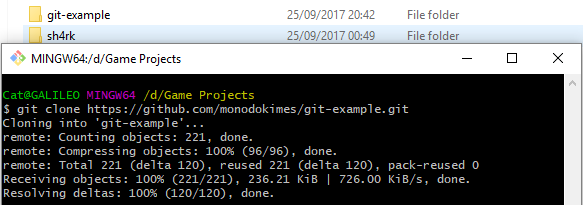
\includegraphics[width=\linewidth]{images/clone.png}
    \caption{Cloning a repository from the command line.}
    \label{fig:clone}
\end{figure}

\paragraph{}
Perfect! Now you're all set up to work in a team, with one final piece of missing knownledge; \texttt{git pull}. When someone makes changes to the project and uses \texttt{git push} to send their work to the server, the other team members won't get the updates immediately. They will, however, run into a brick wall when they try to push their own changes; the server won't let them as the local and remove versions of the project have diverged! We need some way to get the other person's changes and apply them to our local copy of the project. \texttt{git pull} provides this.

\paragraph{}
First, make sure all your local changes are committed (no red or green text when you run \texttt{git status}). Run \texttt{git pull \-r} to get your team's changes and apply them locally. The \texttt{\-r} flag stands for \textit{rebase} - out of scope of this guide, but certainly worth learning about. It's also worth learning about \textit{merges}, especially as you move onto more complex workflows. See \ref{fig:rebase-workflow} for an updated set of commands.

\begin{figure}
    \begin{lstlisting}
        1.  open project
        2.  git pull
        3.  add some changes
        4.  commit them
        5.  git pull -r
        6.  git push
        7.  repeat from step 3
    \end{lstlisting}
    \caption{A basic Git workflow for teams.}
    \label{fig:rebase-workflow}
\end{figure}

\section{Keeping it clean}
As mentioned earlier, usually we don't actually want to track changes to \textit{every} file in your project. Usually it's not only unnecessary but detrimental to performance, clarity and sometimes the portability of the project. IDEs and other tools (in our case, the Unity game engine) generate a lot of files automatically, such as when building. These files don't need to be tracked, so we should find a way to ignore them. This is accomplished using a \texttt{.gitignore} file. This is a file stored in your repository that lets Git know which folders and files are safe to ignore. The contents of your \texttt{.gitignore} will depend on the type of your project. An example for Unity can be found \href{https://github.com/github/gitignore/blob/master/Unity.gitignore}{here}. As you can see, it will ignore all sorts of things but the \texttt{Assets/} and \texttt{ProjectSettings} folders will still be tracked since they contain the user-created files that are needed to build the project.

\paragraph{}
To add one to your project, simply create a file in the root directory of your project called \texttt{.gitignore} (or if you're using Windows, \texttt{.gitignore.txt}, then run the command \texttt{mv .gitignore.txt .gitignore} to rename it. Windows won't allow creation of files without a file extension, not can File Explorer rename a file as such). Find an example online to copy, or write your own, updating the contents of the file with the paths you want to ignore. Save the file.

\paragraph{}
Once you've created an ignore file meeting your requirements, simply add and commit it to the repository as you would any other file. And you're done! No longer will your repository be riddled with bloated commits and unnecessary files.

\section{Before you disappear!}
The material covered in this guide is \textit{very} vague and informal. There's an interactive tutorial on Git \href{https://try.github.io/}{here}. Consult Git's \href{https://git-scm.com/documentation}{official documentation} to learn more about the commands used. If you have any feedback about the guide, please let me know at \href{mailto:me@ktyl.dev}{me@ktyl.dev}. Thanks for reading, and happy committing!

\end{document}
